%%%%%%%%%%%%  Generated using docx2latex.com  %%%%%%%%%%%%%%

%%%%%%%%%%%%  v2.0.0-beta  %%%%%%%%%%%%%%

\documentclass[12pt]{article}
\usepackage{amsmath}
\usepackage{latexsym}
\usepackage{amsfonts}
\usepackage[normalem]{ulem}
\usepackage{soul}
\usepackage{array}
\usepackage{amssymb}
\usepackage{extarrows}
\usepackage{graphicx}
\usepackage[backend=biber,
style=numeric,
sorting=none,
isbn=false,
doi=false,
url=false,
]{biblatex}\addbibresource{bibliography.bib}

\usepackage{subfig}
\usepackage{wrapfig}
\usepackage{wasysym}
\usepackage{enumitem}
\usepackage{adjustbox}
\usepackage{ragged2e}
\usepackage[svgnames,table]{xcolor}
\usepackage{tikz}
\usepackage{longtable}
\usepackage{changepage}
\usepackage{setspace}
\usepackage{hhline}
\usepackage{multicol}
\usepackage{tabto}
\usepackage{float}
\usepackage{multirow}
\usepackage{makecell}
\usepackage{fancyhdr}
\usepackage[toc,page]{appendix}
\usepackage[hidelinks]{hyperref}
\usetikzlibrary{shapes.symbols,shapes.geometric,shadows,arrows.meta}
\tikzset{>={Latex[width=1.5mm,length=2mm]}}
\usepackage{flowchart}\usepackage[paperheight=11.0in,paperwidth=8.5in,left=1.0in,right=1.0in,top=1.0in,bottom=1.0in,headheight=1in]{geometry}
\usepackage[utf8]{inputenc}
\usepackage[T1]{fontenc}
\TabPositions{0.5in,1.0in,1.5in,2.0in,2.5in,3.0in,3.5in,4.0in,4.5in,5.0in,5.5in,6.0in,}

\urlstyle{same}

\renewcommand{\_}{\kern-1.5pt\textunderscore\kern-1.5pt}

 %%%%%%%%%%%%  Set Depths for Sections  %%%%%%%%%%%%%%

% 1) Section
% 1.1) SubSection
% 1.1.1) SubSubSection
% 1.1.1.1) Paragraph
% 1.1.1.1.1) Subparagraph


\setcounter{tocdepth}{5}
\setcounter{secnumdepth}{5}


 %%%%%%%%%%%%  Set Depths for Nested Lists created by \begin{enumerate}  %%%%%%%%%%%%%%


\setlistdepth{9}
\renewlist{enumerate}{enumerate}{9}
		\setlist[enumerate,1]{label=\arabic*)}
		\setlist[enumerate,2]{label=\alph*)}
		\setlist[enumerate,3]{label=(\roman*)}
		\setlist[enumerate,4]{label=(\arabic*)}
		\setlist[enumerate,5]{label=(\Alph*)}
		\setlist[enumerate,6]{label=(\Roman*)}
		\setlist[enumerate,7]{label=\arabic*}
		\setlist[enumerate,8]{label=\alph*}
		\setlist[enumerate,9]{label=\roman*}

\renewlist{itemize}{itemize}{9}
		\setlist[itemize]{label=$\cdot$}
		\setlist[itemize,1]{label=\textbullet}
		\setlist[itemize,2]{label=$\circ$}
		\setlist[itemize,3]{label=$\ast$}
		\setlist[itemize,4]{label=$\dagger$}
		\setlist[itemize,5]{label=$\triangleright$}
		\setlist[itemize,6]{label=$\bigstar$}
		\setlist[itemize,7]{label=$\blacklozenge$}
		\setlist[itemize,8]{label=$\prime$}



 %%%%%%%%%%%%  Header here  %%%%%%%%%%%%%%


\pagestyle{fancy}
\fancyhf{}
\chead{ 
\vspace{\baselineskip}
}
\renewcommand{\headrulewidth}{0pt}
\setlength{\topsep}{0pt}\setlength{\parindent}{0pt}

 %%%%%%%%%%%%  This sets linespacing (verticle gap between Lines) Default=1 %%%%%%%%%%%%%%


\renewcommand{\arraystretch}{1.3}

\title{Privacy-Aware Personalized Advanced Driver-Assistance Systems (ADAS)\vspace{-3em}}
\date{}


%%%%%%%%%%%%%%%%%%%% Document code starts here %%%%%%%%%%%%%%%%%%%%

\begin{document}

\maketitle
\begin{Center}
Armand Ahadi-Sarkani, faculty advisor Professor Salma Elmalaki 
\end{Center}\par

\section{Thesis}
\addcontentsline{toc}{subsection}{Thesis}
Many\ of the current state-of-the-art Advanced Driver Assistance Systems (ADAS) rely solely on sensory and driving data in order to warn or act on behalf of the driver in dangerous situations.  This research project aims to develop an adaptive model based on machine learning and reinforcement learning that is able to quantify and understand various high-level human states. These human states will then be used in conjunction with data received from ADAS on vehicles to personalize and improve the relevance of warnings and actions that are taken by these systems. The measurements taken on the human state will be context-aware, and thus place a significant importance on respecting the privacy of users.\par

\section{Purpose}
\addcontentsline{toc}{subsection}{Purpose }
Many of the current state-of-the-art Advanced Driver Assistance Systems (ADAS) rely on data received from sensors mounted on vehicles, in addition to driving data and telemetry generated with the motion of the vehicle and driver actions. Examples of such driver assistance systems employed on modern vehicles include lane departure warning, forward collision warning, and braking assistance systems. These driver assistance systems only rely on quantifiable, generic data from the vehicle or the environment in which the vehicle is operating. \par

%% repetition
\vspace{\baselineskip}
The motivation behind this research project is to explore the question of whether or not these systems can be improved by introducing the element of the human state into their decision-making process. This proposed improvement can result in driver assistance systems that are more tailored to the state of mind, health, and predicted behavior of individuals. Additionally, this research project aims to make these systems privacy-aware, ensuring that personal data collected about a human’s state does not get shared.\par


\vspace{\baselineskip}
The field of introducing human-in-the-loop interaction to systems is still in its growing stages, and is yet to be effectively applied to real-world scenarios that the general public encounters on a daily basis. Promoting safer driving and preventing dangerous road events through driver assistance systems is a top concern for engineers in this field. Introducing greater human interaction in the decision-making process of these systems will help advance this cause.\par

\section{Objective}
\addcontentsline{toc}{subsection}{Objective}
This\ research project aims to first understand how this sensory and telemetric data is collected to create ADAS systems, by using a modern, autonomous driving simulation environment. The simulation environment of choice is CARLA Simulator, an open-source simulator designed for autonomous driving research, based on the OpenDrive standard. \par %% last sentence reword discuss preliminary results

%% separate first and second methods into subsections, and subsection for future work

\vspace{\baselineskip}
The first stages of this research project involved learning about CARLA Simulator and the various APIs and sensors available. The primary task completed was creating a lane departure warning, ADAS sensor using CARLA APIs and simulating the effects of this sensor using various driving scenarios, both autonomous and involving manual control of the vehicle. In order to explore how lane departure sensors work, this task was performed using two means, and comparing the experimental results of each.\par


\subsection{Visual-based lane departure warning}
%%%%%%%%%%%%%%%%%%%% Figure/Image No: 1 starts here %%%%%%%%%%%%%%%%%%%%

\begin{figure}[H]
\centering
\begin{subfigure}
\captionof{figure}{Output of semantic segmentation camera}
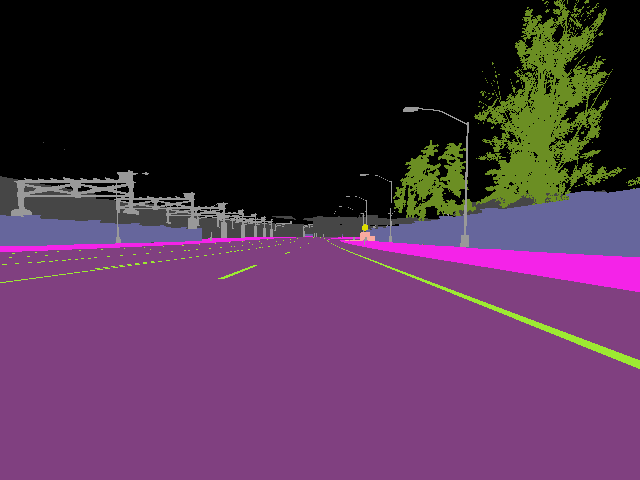
\includegraphics[width=0.45\textwidth]{./media/image1.png}
\end{subfigure}
\begin{subfigure}		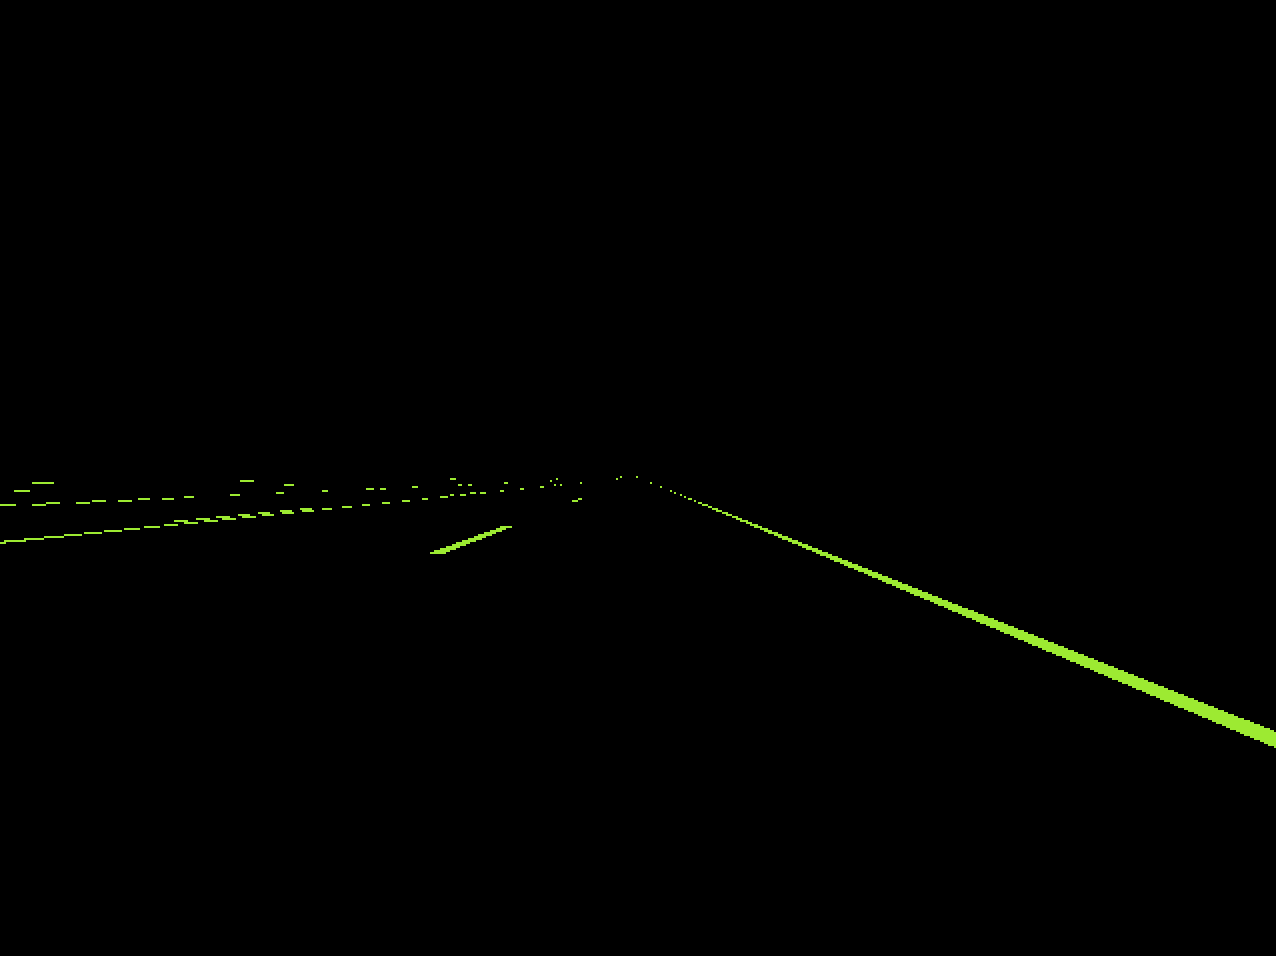
\includegraphics[width=0.45\textwidth]{./media/image2.png}
\end{subfigure}
\end{figure}


%%%%%%%%%%%%%%%%%%%% Figure/Image No: 1 Ends here %%%%%%%%%%%%%%%%%%%%

\hspace{2cm} \textbf{(a) } Unmasked output \hspace{2.75cm} \textbf{(b) }Roadline-masked output \par
\vspace{\baselineskip}
The first method of creating a lane departure warning sensor in CARLA involves visually interfacing with the built-in cameras available to vehicles in the simulation environment. The ideal camera for this is the semantic segmentation camera, which classifies different pixels in an image into multiple classes based on their meaning in the environment in which they reside. In CARLA, such classes of pixels include those that reference buildings, pedestrians, poles, vehicles, traffic signs, or roadlines. The roadline data is used in this implementation to capture data about the location of lane markings and how they change as the vehicle is in motion.\textbf{ Figure 1A} shows the standard output of the semantic segmentation camera taken in a customizable driving scenario. As images like \textbf{figure 1A }were received by the semantic segmentation camera, a masking algorithm was applied in order to hide all classes of pixels that did not correspond to roadlines. \textbf{Figure 1B }shows the output of that masking algorithm applied onto \textbf{figure 1A}, only showing the CARLA defined $``$roadlines$"$ , or lane markings. This masking was applied in order to establish a basis for a lane departure warning system. This system operates by computing the difference between multiple masked frames at once (initially set at \textit{n = 2} frames) from the continuous sequence of frames received from the camera as the vehicle is in motion. Multiple linear algebra-based algorithms have been employed to compute this difference, as well as interfacing with APIs from SciPy. This visual method for creating a lane-departure warning ADAS system is a work in progress.\par

\subsection{Location-based lane departure warning}

%%%%%%%%%%%%%%%%%%%% Figure/Image No: 2 starts here %%%%%%%%%%%%%%%%%%%%

\begin{figure}[H]
\captionof{figure}{Location of lane markings on CARLA server}
\centering
\advance\leftskip 0.0in		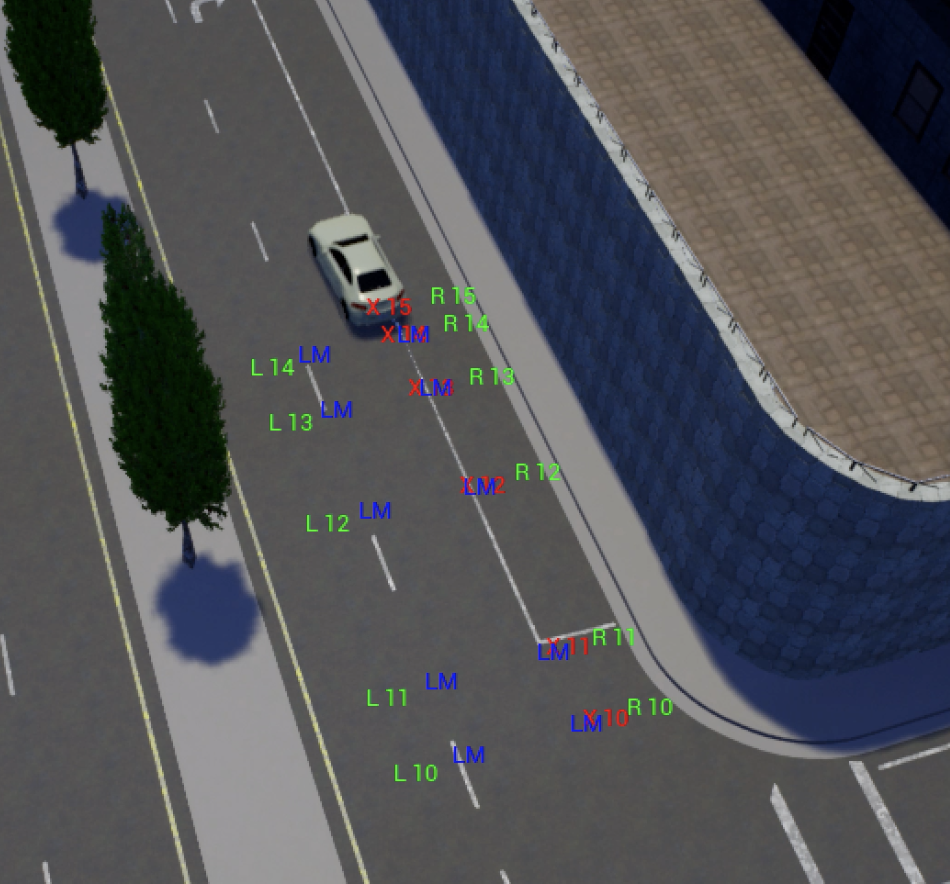
\includegraphics[width=3.65in,height=3.39in]{./media/image3.png}
\par
\vspace{\baselineskip}
\end{figure}


%%%%%%%%%%%%%%%%%%%% Figure/Image No: 2 Ends here %%%%%%%%%%%%%%%%%%%%

\vspace{\baselineskip}
The second method of creating a lane departure warning sensor using CARLA involves analyzing vehicle location data in comparison with pre-defined waypoint data provided by the simulator. CARLA waypoints are vector-like objects that describe points in a road and provide information about the location and size of lanes. By continuously polling the location of the vehicle and relaying waypoint data about the nearest left and right lanes to the vehicle, an algorithm was created in order to determine the position of lane markings and \tab  how they relate to the vehicle in motion. \textbf{Figure 2 }shows the calculated locations of lane markings (blue), centers of right and left lanes (green), and the vehicle’s location (red) on a simulator window, as a vehicle is in motion. If the vehicle is steering towards any of these lane markings on its right or left side, and reaches a preset threshold between these lane markings, a warning is engaged. This method is implemented through a client-server model; the client program is a manually-controlled driving environment, relaying waypoint and location data to the server program, which remotely is able to compute whether or not the vehicle in motion is approaching a lane marking. If the vehicle is approaching a lane from its left or right side, the server program sends a warning to the client. This client program is by default relaying data to the server at around 60 times per second, and the server program is able to filter that data and sample it for computation at a pre-defined sampling rate.\par

\subsection{Future objectives}
In the near-term, the visual lane departure warning system (using the semantic segmentation camera) will be improved, with an intention to provide a candidate basis for integrating personalized, human interaction-based learning into existing ADAS systems. The second method, involving analyzing vehicle location and waypoint data, will also be improved, by implementing other vehicle data (such as velocity, acceleration, and steering trajectories) that would be necessary in categorizing the various human driver states (such as aggressive, drowsy, and inattentive driving). Medium-term objectives of this project include creating other ADAS sensors (such as forward collision warning), and integrating key hardware such as sensors and monitors that are able to relay data about a human’s mood, health, and well-being. This will help, in the long-term, to introduce a model that is able to interface with this data in order to develop adaptive ADAS systems that learn from data about the human state, and ultimately integrate privacy-aware data collection.\par

\section{Approach}
\addcontentsline{toc}{subsection}{Approach}
This project will primarily involve developing algorithms and models with the help of open-source software, such as CARLA Simulator. CARLA will be the primary simulation environment that will be interfaced with in this project, due to its versatility and variety of available driving environments. Longer-term goals involve integrating the aforementioned hardware into CARLA to communicate data about the human state with the ADAS sensors that have been created. \par


\vspace{\baselineskip}
The\ research process will involve interacting with various mediums including hardware and  simulation environments. Due to the ability to create comprehensive models of the human state with the help of this hardware, simulations, and no outside human subjects, this project is feasible without exorbitant funding beyond UROP grants, and given the remote learning situation likely to occur during the Fall quarter. \par


\vspace{\baselineskip}
This project will be conducted under the Campuswide Honors Collegium’s undergraduate research guidance, and thus a comprehensive thesis will be written at its completion.\par

\section{Responsibilities}
\addcontentsline{toc}{subsection}{Responsibilities}
This project is individual and not group-based. Armand Ahadi-Sarkani assumes full responsibility for all research work, under the guidance of Prof. Salma Elmalaki, Assistant Professor of Teaching in the Electrical Engineering and Computer Science department.\par

\section{Timeline}
\addcontentsline{toc}{subsection}{Timeline}

\vspace{\baselineskip}
\vspace{-1em}


%%%%%%%%%%%%%%%%%%%% Table No: 1 starts here %%%%%%%%%%%%%%%%%%%%


\begin{table}[H]
 			\centering
\begin{tabular}{p{4.05in}p{2.05in}}
\hline
%row no:1
\multicolumn{1}{|p{4.05in}}{\cellcolor[HTML]{B7B7B7}\textbf{Objective}} & 
\multicolumn{1}{|p{2.05in}|}{\cellcolor[HTML]{B7B7B7}\textbf{Estimated Completion}} \\
\hhline{--}
%row no:2
\multicolumn{1}{|p{4.05in}}{Improving metrics for lane departure warning system} & 
\multicolumn{1}{|p{2.05in}|}{June 2020} \\
\hhline{--}
%row no:3
\multicolumn{1}{|p{4.05in}}{Purchasing and collecting data from hardware sensors } & 
\multicolumn{1}{|p{2.05in}|}{June - August 2020} \\
\hhline{--}
%row no:4
\multicolumn{1}{|p{4.05in}}{Interfacing hardware sensors with CARLA Simulator} & 
\multicolumn{1}{|p{2.05in}|}{July - August 2020} \\
\hhline{--}
%row no:5
\multicolumn{1}{|p{4.05in}}{Integrating human state data and creating learned, personalized models for ADAS systems} & 
\multicolumn{1}{|p{2.05in}|}{Fall Quarter 2020} \\
\hhline{--}
%row no:6
\multicolumn{1}{|p{4.05in}}{Complete Campuswide Honors Thesis} & 
\multicolumn{1}{|p{2.05in}|}{Winter Quarter 2021} \\
\hhline{--}

\end{tabular}
 \end{table}


%%%%%%%%%%%%%%%%%%%% Table No: 2 ends here %%%%%%%%%%%%%%%%%%%%

\section{Works Cited}
\addcontentsline{toc}{subsection}{Works Cited}
\setlength{\parskip}{12.0pt}
Em, Poh Ping, et al. $``$Vision-Based Lane Departure Warning Framework.$"$  \textit{Heliyon}, Elsevier, 6 Aug. 2019, \href{http://www.ncbi.nlm.nih.gov/pmc/articles/PMC6698973/}{\textcolor[HTML]{1155CC}{\ul{www.ncbi.nlm.nih.gov/pmc/articles/PMC6698973/}}}.\par

$``$Lane-Keeping-Assist-on-CARLA.$"$  \textit{GitHub}, \href{http://www.github.com/paulyehtw/Lane-Keeping-Assist-on-CARLA}{\textcolor[HTML]{1155CC}{\ul{www.github.com/paulyehtw/Lane-Keeping-Assist-on-CARLA}}}.\par

$``$CARLA Simulator.$"$  \textit{GitHub, \href{http://www.github.com/carla-simulator/carla}{}\textcolor[HTML]{1155CC}{\ul{www.github.com/carla-simulator/carla}}}\par

Elmalaki, Salma, et al. $``$Sentio: Driver-in-the-Loop Forward Collision Warning Using Multisample Reinforcement Learning.$"$  \textit{Sentio $ \vert $  Proceedings of the 16th ACM Conference on Embedded Networked Sensor Systems}, 1 Nov. 2018, \href{http://www.dl.acm.org/doi/10.1145/3274783.3274843}{\textcolor[HTML]{1155CC}{\ul{www.dl.acm.org/doi/10.1145/3274783.3274843}}}.\par

$``$SciPy.$"$  \textit{SciPy, \href{http://www.scipy.org}{}\textcolor[HTML]{1155CC}{\ul{www.scipy.org}}}\par


\vspace{\baselineskip}

\vspace{\baselineskip}

\vspace{\baselineskip}

\vspace{\baselineskip}

\vspace{\baselineskip}

\vspace{\baselineskip}

\vspace{\baselineskip}

\vspace{\baselineskip}

\vspace{\baselineskip}

\vspace{\baselineskip}

\vspace{\baselineskip}

\vspace{\baselineskip}

\vspace{\baselineskip}

\vspace{\baselineskip}

\printbibliography
\end{document}